% =====================================================================
% foto_capa.tex -- Segunda pagina estilizada (estilo capa de revista,
% referencia: capa "Energia Nuclear" da FGV Energia), usando a foto
% aerea do RMB.
% =====================================================================
\clearpage
\newgeometry{top=1.6cm,bottom=2.5cm,left=3.0cm,right=2.3cm}
\thispagestyle{empty}
\setlength{\parindent}{0pt}
\singlespacing

% ---- Barra superior: identificacao + linha de "edicao" ----
\noindent
\begin{minipage}[c]{0.28\textwidth}
{\sffamily\bfseries\large CNEN\,\textbar\,RMB}
\end{minipage}%
\begin{minipage}[c]{0.02\textwidth}
\centering\color{nurule}\rule{0.7pt}{18pt}
\end{minipage}%
\begin{minipage}[c]{0.70\textwidth}
\raggedleft\sffamily\small
REV.\ B~~\textbar~~RPAS -- CAP\'ITULO 1~~\textbar~~SETEMBRO 2026
\end{minipage}

\vspace{4pt}
\color{nurule}\rule{\textwidth}{1.4pt}

\vspace{10pt}

% ---- Foto de largura total ----
\noindent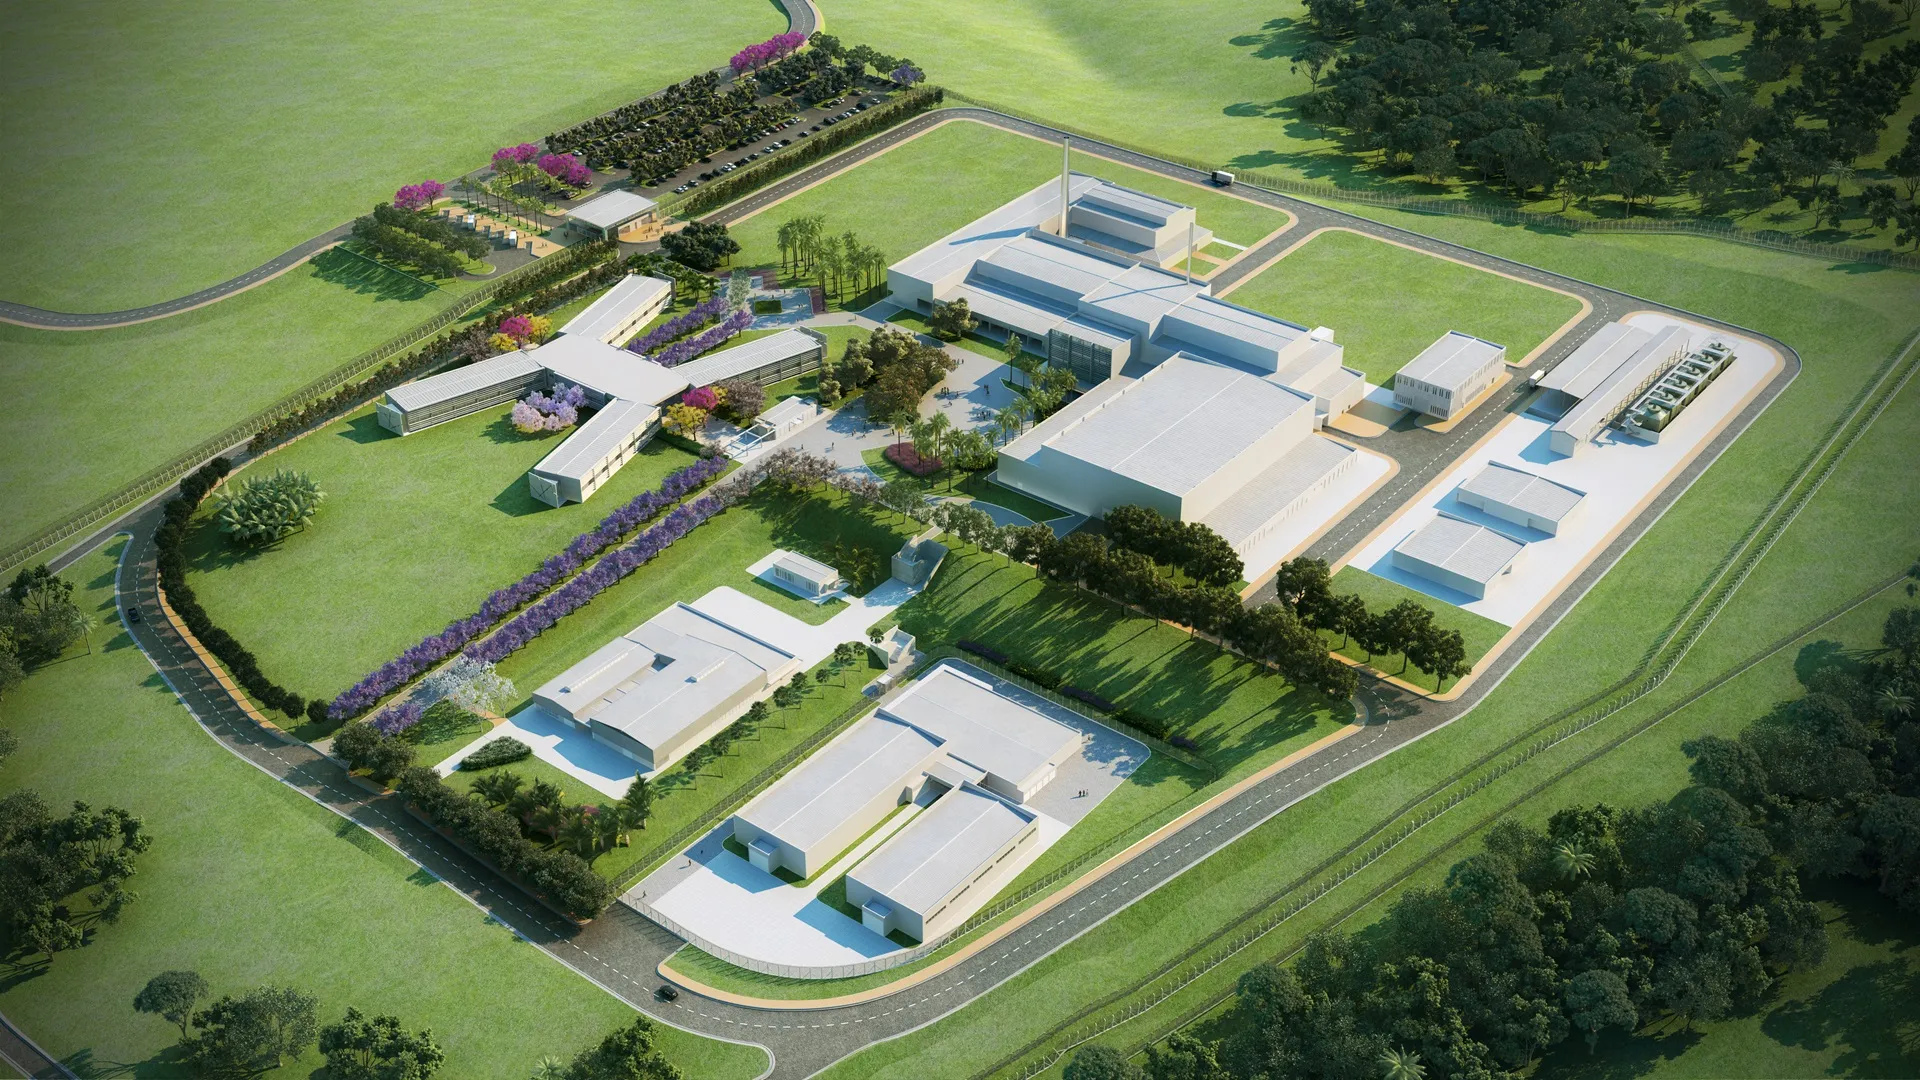
\includegraphics[width=\textwidth]{figures/rmb_vista_aerea.png}

\vspace{16pt}

% ---- Titulo grande, estilo capa de revista ----
\begin{center}
{\sffamily\bfseries\fontsize{24}{28}\selectfont\color{nurule}
REATOR MULTIPROP\'OSITO BRASILEIRO}\\[10pt]
{\sffamily\large RELAT\'ORIO PRELIMINAR DE AN\'ALISE DE SEGURAN\c{C}A}
\end{center}

\vfill
{\small\color{nugray}\itshape Vista a\'erea do complexo do RMB -- Ipero/SP (imagem ilustrativa do projeto).}\\[4pt]
\color{nurule}\rule{\textwidth}{0.6pt}
\restoregeometry
\clearpage
